\subsection{Finite Field Dependency}
\label{sec:implementation__dependencies}
\label{sec:implementation_dependency}

\begin{figure}
	\centering
	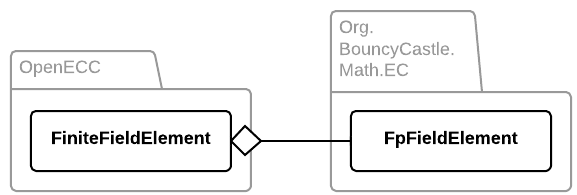
\includegraphics[width=0.7\textwidth]{implementation/finitefields}
	\caption{The \texttt{FiniteFieldElement} is simply a wrapper around \texttt{Org.BouncyCastle.Math.EC.FpFieldElement},
		BouncyCastle's Finite Field implementation. It takes care of conversion between C\#'s native \texttt{BigIntegers} and
		BouncyCastle's own \texttt{BigInteger} implementation.}
\end{figure}

\textbf{Note: Review this section, ensure focus. Focus should be on the trouble of BigIntegers, and how
this may be significantly damaging to performance. Then link to performance section where this is looked into.}

\textbf{Note: the wrapper provides nice syntax, show the difference between bouncycastle's addition of points
and ours.}

An integral part of Elliptic Curve (and much other) cryptography is finite fields and arithmetic
over finite fields. Per default no such functionality exists in C\#.

Bouncy Castle contains, among other things, an implementation of finite fields, that is also used
in the \emph{OpenECC} implementation.

Integrating just the \verb+Org.BouncyCastle.Math.EC.FpFieldElement+ (finite field implementation) into
the project is not trivial, however, as it uses a BigInteger implementation defined in BouncyCastle,
which differs from that in C\#'s System.Numerics.BigInteger.

To solve these issues, a wrapper (FiniteFieldElement) was created. This wrapper maps from BouncyCastle's
BigIntegers to the normal BigIntegers, reducing the boilerplate between BouncyCastle and OpenECC to
just one class.

The primary problem here is converting between the two BigInteger implementations\footnote{This seems
to be a previously unsolved problem, which has previously been posed (http://stackoverflow.com/questions/21756578/how-do-i-round-trip-a-number-to-bouncycastle-biginteger-system-numerics-big)}.
In this implementation the string forms of the BigIntegers have been used to convert.

\begin{verbatim}
	...ToBouncyCastleBigInteger(this System.Numerics.BigInteger i)...
	return new Org.BouncyCastle.Math.BigInteger(i.ToString());
	
	...
	
	...ToNativeBigInteger(this Org.BouncyCastle.Math.BigInteger i)...
	return System.Numerics.BigInteger.Parse(i.ToString());
\end{verbatim}

This, admittedly, is far from efficient, but as there is little documentation of the byte-level structure
of Bouncy Castle's BigIntegers the performance sacrifice was deemed preferable. The performance implications
of this are covered in Section \ref{sec:performance}.